\chapter{Physics behind numerical methods}\label{Formulae}

\section{Distribution function transform}
Distribution function of particles in phase space is presented in code in spherical coordinates $n(\epsilon,\mu,\phi)$. Let consider transform to the frame moving along $z$-axis with lorentz-factor $\gamma = 1/\sqrt{1-\beta^2}$. Number of particles in the corresponding phase volumes $N$ is invariant.

\begin{equation}
	N = n(\epsilon,\mu,\phi)d\epsilon d\mu d\phi dV = n'(\epsilon',\mu',\phi')d\epsilon' d\mu' d\phi' dV'
\end{equation}

So, to obtain $n'$ we need to evaluate determinant of Jacobi transformation matrix. Note, that aximuthal angle phi does not changes in transformation to the moving frame $phi' = phi$, and energy and polar angle does not depend on space volume, so in general Jacobi matrix has following non-zero terms

\begin{equation}\label{generalJacobi}
	J=\left(
	\begin{array}{cccc}
		\frac{d\epsilon'}{d\epsilon} & \frac{d\epsilon'}{d\mu}& 0 & 0\\
		\frac{d\mu'}{d\epsilon} & \frac{d\mu'}{d\mu} & 0 & 0\\
		0 & 0 & 1 & 0\\
		\frac{dV'}{d\epsilon} & \frac{dV'}{d\mu} & 0 & \frac{dV'}{dV}
	\end{array}
	\right)
\end{equation}

Let start with transforming space volume $V$. First approach, following Landau-Lifshitz 2, paragraph 10 \cite{LandauLifshitz2}, is to transform volume to the rest-frame of moving beam of particle with given momentum, and then derive that $dV'/dV= \epsilon/\epsilon'$. It is correct result, but proof is not valid for massles particles, which have not physical rest frame.

So we evaluate transformation of volume, containing chosen particles, directly from Lorentz transformations. Let assume flux of particles, aligned with z axis, with uniform interval $L$ between them, moving with same velocity $v$ with angle $\theta$ to the z axis, and $\mu = cos(\theta)$, as it is shown in Figure \ref{VolumeTransform}.

\begin{figure}[h]
	\centering
	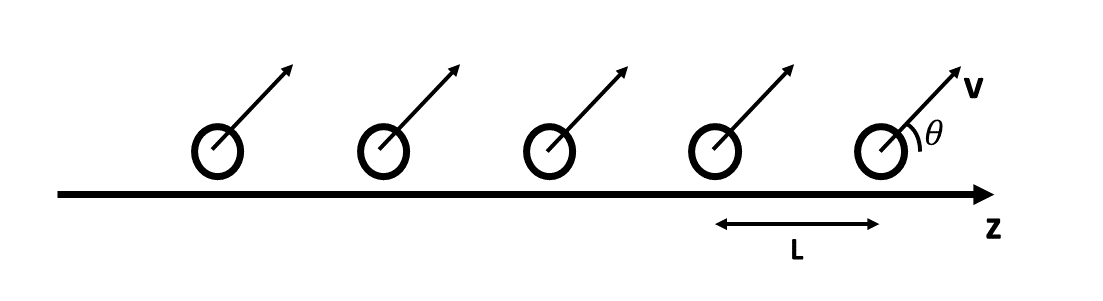
\includegraphics[width=12.5 cm]{./fig/VolumeTransform.png} 
	\caption{Beam of evenly distributed particles}
	\label{VolumeTransform}
\end{figure}

So in the lab frame, at the moment $t$ i-th particle is placed at $z_i = i\cdot L + \mu v t$. Let evaluate coordinates of particles in the moving frame.

\begin{equation}\label{lorentz_z}
	\left(\begin{array}{c}
		ct'\\
		z'_i
	\end{array}
	\right)
	= \left(
	\begin{array}{cc}
		\gamma & -\beta\gamma\\
		-\beta\gamma & \gamma
	\end{array}
	\right)
	\times
	\left(\begin{array}{c}
		ct\\
		z_i
	\end{array}
	\right)
\end{equation}

From this we can obtain values $z'_i = \gamma z_i + (\gamma \mu v - c\beta \gamma)t$, but this values are measured at the different time moments in the moving frame, if $t$ is the same for all particles in lab frame. To evaluate volume or number density we should evaluate them at the same moment $t'$. So let express $t$ in terms of $z_i$ and $t'$, and put into the equation for $z'_i$.

\begin{equation}
	t=\frac{t'+\gamma\beta z_i/c}{\gamma - \beta \mu v/c}
\end{equation}

and

\begin{equation}
	z'_i=\gamma z_i +(\gamma \mu v - c\beta \gamma)\frac{t'+\gamma\beta z_i/c}{\gamma - \beta \mu v/c}=z_i\frac{1}{\gamma(1-\beta\mu v/c)} + t'\frac{\mu v/c - \beta}{1 - \beta \mu v/c}
\end{equation}

Second term, containing $t'$ gives us standard  relativistic velocity-addition formula. And the first one gives a desired expression to the compression of the distance between particles. $L' = z'_{i+1}-z'_i = L/(\gamma(1-\beta\mu v/c))$. The distances in the transversal directions does not comress with Lorentz transformations, so volume also transforms as
\begin{equation} \label{volume}
V' = V/(\gamma(1-\beta\mu v/c))
\end{equation}
This result is the same, as given by \cite{LandauLifshitz2}.

Next, we need to find expressions for $\epsilon'$ and $\mu'$, but it is better to deal with them in to separate cases - for massless and massive particles.

\subsection{Photons}
For massles photons, we consider transformation of energy-mometum vector, taking into account that $z$ component of momentum is $p_z = \mu \epsilon/c$, and transversal components stay constant.

\begin{equation}\label{lorentz_ph}
	\left(\begin{array}{c}
		\epsilon'\\
		\mu'\epsilon'
	\end{array}
	\right)
	= \left(
	\begin{array}{cc}
		\gamma & -\beta\gamma\\
		-\beta\gamma & \gamma
	\end{array}
	\right)
	\times
	\left(\begin{array}{c}
		\epsilon\\
		\mu\epsilon
	\end{array}
	\right)
\end{equation}

From the first line we get equation for doppler shift of photon's energy

\begin{equation}\label{doppler_ph}
	\epsilon'=\gamma(1-\mu\beta)\epsilon
\end{equation}

Derivatives of $\epsilon'$ with respect to $\epsilon$ and $\mu$ are

\begin{equation}
	\frac{d\epsilon'}{d\epsilon}=\gamma(1-\mu\beta)
\end{equation}

\begin{equation}
	\frac{d\epsilon'}{d\mu}=-\gamma\beta\epsilon
\end{equation}

From the second line of \ref{lorentz_ph} we get
 $\mu'\epsilon'=-\beta\gamma\epsilon+\gamma\mu\epsilon$. Then we plug in expression for $\epsilon'$ from \ref{doppler_ph} and obtain equation for aberration of light
 
\begin{equation}\label{aberration_ph}
	\mu'=\frac{\mu-\beta}{1-\mu\beta}
\end{equation}

Angle of photon's velocity to the z-axis does not depend on their energy. And derivative of $\mu'$ with respect to $\mu$ is

\begin{equation}
	\frac{d\mu'}{d\mu} = \frac{d\mu'}{d\mu}=\frac{d}{d\mu}\frac{1}{\beta}\frac{\beta\mu-1+1-\beta^2}{1-\mu\beta}=\frac{d}{d\mu}\frac{1}{\beta}\frac{1-\beta^2}{1-\mu\beta}=\frac{1-\beta^2}{(1-\mu\beta)^2}=\frac{1}{\gamma^2(1-\mu\beta)^2}
\end{equation}

And Jacobi matrix of coordinate transformation in case of photons is
\begin{equation}
	J=\left(
	\begin{array}{cccc}
		\frac{d\epsilon'}{d\epsilon} & \frac{d\epsilon'}{d\mu}& 0 & 0\\
		0 & \frac{d\mu'}{d\mu} & 0 & 0\\
		0 & 0 & 1 & 0\\
		0 & \frac{dV'}{d\mu} & 0 & \frac{dV'}{dV}
	\end{array}
	\right)
\end{equation}

Determinant of thos matrix, fortunately, equals to the multiple of diagonal terms

\begin{equation}\label{jacobian_ph}
	\frac{D(\epsilon',\mu',\phi',V')}{D(\epsilon,\mu,\phi,V)}=\frac{d\epsilon'}{d\epsilon}\frac{d\mu'}{d\mu}\frac{dV'}{dV}=\gamma(1-\mu\beta)\frac{1}{\gamma^2(1-\mu\beta)^2}\frac{1}{\gamma(1-\mu\beta)}=\frac{1}{\gamma^2(1-\mu\beta)^2}
\end{equation}

And finally, photons distribution function in spherical coordinates transforms as
\begin{equation}\label{distribution_ph}
	n'_{ph}(\epsilon',\mu',\phi') = \frac{n_{ph}(\epsilon,\mu,\phi)}{\frac{D(\epsilon',\mu',\phi',V')}{D(\epsilon,\mu,\phi,V)}}=\gamma^2(1-\mu\beta)^2 n_{ph}(\epsilon,\mu,\phi)
\end{equation}
\subsection{Massive particles}
In the case of massive particles, expression for $\epsilon'$ and $\mu'$ are more complicated. Now $p_z = \mu \sqrt{\epsilon^2 - m^2 c^4}/c$, where $m$ is particle mass, and Lorentz transformation of energy-momentum vector is expressed as

\begin{equation}\label{lorentz_m}
	\left(\begin{array}{c}
		\epsilon'\\
		\mu'\sqrt{{\epsilon'}^2 - m^2 c^4}
	\end{array}
	\right)
	= \left(
	\begin{array}{cc}
		\gamma & -\beta\gamma\\
		-\beta\gamma & \gamma
	\end{array}
	\right)
	\times
	\left(\begin{array}{c}
		\epsilon\\
		\mu\sqrt{{\epsilon}^2-m^2 c^4}
	\end{array}
	\right)
\end{equation}

So expressions for $\epsilon'$ and $\mu'$ are

\begin{equation}
	\epsilon' = \gamma\epsilon-\beta\gamma\mu\sqrt{\epsilon^2-m^2 c^4}
\end{equation}
\begin{equation}
	\mu' = \frac{-\beta\gamma\epsilon+\gamma\mu\sqrt{{\epsilon}^2-m^2 c^4}}{\sqrt{{\epsilon^2 - m^2 c^4}}}
\end{equation}

And expresson for volume transformation \ref{volume} in terms of $\epsilon$ and $\mu$ is
\begin{equation}
	V'=\frac{V}{\gamma(1-\mu\beta\sqrt{{\epsilon}^2-m^2 c^4}/\epsilon)}
\end{equation}

Expressions for partial derivatives of $\epsilon'$, $\mu'$, $V'$, and especially for Jacobian are really terrible, so here we present only final result for distribution function in units $c = 1$

\begin{equation}
		\frac{n'_{m}(\epsilon',\mu',\phi')}{n_{m}(\epsilon,\mu,\phi)}= \frac{\gamma(\epsilon-\mu\sqrt{{\epsilon}^2-m^2}\beta)(\gamma^2\epsilon^2-m^2 + \mu^2 ((\epsilon^2-m^2)(\gamma^2-1)) - 2\mu\epsilon\gamma^2\beta\sqrt{\epsilon^2-m^2})^{3/2}}{\epsilon(((\gamma^2-1)(\epsilon^2-m^2)\mu^2 + \gamma^2\epsilon^2 - m^2)\sqrt{\epsilon^2-m^2}-2\mu\epsilon\gamma(\epsilon^2 - m^2)\sqrt{\gamma^2 - 1})}
\end{equation}

\section{Комптоновское рассеяние}\label{comptonFormulaSection}
Рассмотрим рассеяние фотонов на одном электроне, движущемся вдоль ось z, см \cite{Dubus}. Сечение Клейна-Нишины в системе покоя электрона равно
\begin{equation}
	\frac{d\sigma}{d\epsilon_1'd\Omega_1'}=\frac{{r_e}^2}{2}\left(\frac{\epsilon_1'}{\epsilon_0'}\right)^2(\frac{\epsilon_1'}{\epsilon_0'}+\frac{\epsilon_0'}{\epsilon_1'}-\sin^2\Theta') \delta(\epsilon_1' - \frac{\epsilon_0'}{1+\frac{\epsilon_0'}{m_e c^2}(1 - \cos \Theta')})
\end{equation}
Где $r_e$ - классический радиус электрона, $\epsilon_0'$ и $\epsilon_1'$ - энергии начального и конечного фотона, соответственно, $\Theta'$ - угол между начальным и конечным фотоном, определяемый выражением $\cos\Theta' =\cos \theta_0' \cos \theta_1' + \sin \theta_0' \sin \theta_1' \cos(\phi_1' - \phi_0')$. Штрихованные индексы относятся к системе отсчета электрона. При этом начальная и конечная энергии фотонов оказываются связаны соотношениями
\begin{equation}
	\epsilon_1'=\frac{\epsilon_0'}{1+\frac{\epsilon_0'}{m_e c^2}(1 - \cos \Theta')}	
\end{equation}
\begin{equation}
	\epsilon_0'=\frac{\epsilon_1'}{1-\frac{\epsilon_1'}{m_e c^2}(1 - \cos \Theta')}
\end{equation}
Число фотонов, рассеявшихся в заданный телесный угол в единицу времени в промежуток энергии в системе покоя электрона равно
\begin{equation}
\frac{dN'}{dt'd\epsilon_1'd\Omega_1'}=\int c \frac{d\sigma}{d\epsilon_1'd\Omega_1'} \frac{dn'}{d\epsilon_0'd\Omega_0'}d\Omega_0'd\epsilon_0'
\end{equation}

Перепишем дельта-функцию через энергию начального фотона с помощью соотношения 
\begin{equation}
	\delta(f(x)) = \sum \frac{\delta(x-x_k)}{|f'(x_k)|}
\end{equation}
где $x_k$ - корни функции $f(x)$. Производная выражения внутри дельта-функции равна
\begin{equation}
	\frac{d\epsilon_1'}{d\epsilon_0'}=\frac{1}{(1+\frac{\epsilon_0'}{m_e c^2}(1 - \cos \Theta'))^2}
\end{equation}
и она сократится с квадратом отношения энергий в формуле для сечения. Функцию распределения начальных фотонов выразим в лабораторной системе с помощью выражения \ref{distribution_ph}.
\begin{equation}
	\frac{dN'}{dt'd\epsilon_1'd\Omega_1'}=\int \frac{r_e^2 c}{2} \gamma_e^2 (1 - \mu_0 \beta_e)^2 (\frac{\epsilon_1'}{\epsilon_0'}+\frac{\epsilon_0'}{\epsilon_1'}-\sin^2\Theta')\frac{dn}{d\epsilon_0 d\Omega_0} \delta(\epsilon_0' - \frac{\epsilon_1'}{1-\frac{\epsilon_1'}{m_e c^2}(1 - \cos \Theta')}) d\epsilon_0'd\mu_0' d\phi_0'
\end{equation}
Теперь избавимся от дельта-функции, проинтегрировав по $\epsilon_0'$.
\begin{equation}
	\frac{dN'}{dt'd\epsilon_1'd\Omega_1'}=\int \frac{r_e^2 c}{2} \gamma_e^2 (1 - \mu_0 \beta_e)^2 (1 + \cos^2\Theta'+(\frac{\epsilon_1'}{m_e c^2})^2\frac{(1-\cos\Theta')^2}{1-\frac{\epsilon_1'}{m_e c^2}(1 - \cos \Theta')})\frac{dn}{d\epsilon_0 d\Omega_0}d\mu_0' d\phi_0'
\end{equation}
Осталось перевести поток рассеяных фотонов в лабораторную систему отсчета $\frac{dN}{dt d\epsilon_1 d\Omega_1} = \frac{dN'}{dt' d\epsilon_1' d\Omega_1'}\frac{dt'}{dt}\frac{d\epsilon_1'}{d\epsilon_1}\frac{d\Omega_1'}{d\Omega_1}$. Используя то, что $dt = \gamma_e dt'$, $\epsilon = \frac{1}{\gamma_e(1 -\mu_1\beta_e)}\epsilon'$ и $\mu_1' = \frac{\mu_1-\beta_e}{1-\mu_1 \beta_e}$ получим
\begin{equation} \label{compton_elframe}
	\frac{dN}{dt d\epsilon_1 d\Omega_1}=\int \frac{r_e^2 c}{2} \frac{(1 - \mu_0 \beta_e)^2}{1-\mu_1\beta_e} (1 + \cos^2\Theta'+(\frac{\epsilon_1'}{m_e c^2})^2\frac{(1-\cos\Theta')^2}{1-\frac{\epsilon_1'}{m_e c^2}(1 - \cos \Theta')})\frac{dn}{d\epsilon_0 d\Omega_0}d\mu_0' d\phi_0'	
\end{equation}
При интегрировании нужно выразить углы в лабораторной системе отсчета $\mu_0, \phi_0$ через переменные интегрирования $\mu_0', \phi_0'$. Для расчета рассеяния на распределении электронов нужно проинтегрировать формулу \ref{compton_elframe} с функцией распределения электронов, нормированной на количество частиц. При этом надо учесть разные направления движения электронов и произвести повороты углов.

Так же может быть удобно интегрировать в переменных лабораторной системы расчета, тогда выражение для потока фотонов будет следующим
\begin{equation}\label{compton_labframe}
	\frac{dN}{dt d\epsilon_1 d\Omega_1}=\int \frac{r_e^2 c}{2} \frac{1}{\gamma_e^2(1-\mu_1\beta_e)} (1 + \cos^2\Theta'+(\frac{\epsilon_1'}{m_e c^2})^2\frac{(1-\cos\Theta')^2}{1-\frac{\epsilon_1'}{m_e c^2}(1 - \cos \Theta')})\frac{dn}{d\epsilon_0 d\Omega_0}d\mu_0 d\phi_0
\end{equation}
При рассмотрении процессов, связанных с электронами высоких энергий $\gamma_e \approx 10^8$ относительные численные погрешности вычислений могут быть очень велики, так как $\beta_e$ и $\mu_0, \mu_1, \cos \Theta'$ оказываются слишком близки к единице и стандартный тип double может не разрешать это отличие. Поэтому для численных вычислений оказывается полезным ввести следующие вспомогательные величины:
\begin{equation}
	\delta_e = 1 - \beta_e
\end{equation}
\begin{equation}
	\text{versin}~\theta = 1 - \cos \theta
\end{equation}
Тогда выражения вида $1 - \mu \beta_e$ в этих величинах перепишется как
\begin{equation}
	1 - \mu \beta_e =\text{versin}~\theta + \delta_e - \text{versin}~\theta~\delta_e
\end{equation}
а выражение для угла между конечным и начальным фотоном как
\begin{equation}
	1 - \cos \Theta' = \text{versin}~\theta_0' + \text{versin}~\theta_1' - \text{versin}~ \theta_0' \text{versin}~\theta_1' - \sin \theta_0'\sin \theta_1' \cos(\phi_1'-\phi_0')
\end{equation}
С использованием данных выражений значительно повышается точность и максимальные доступные к рассмотрению энергии фотонов и электронов.

В случае изотропных функций распределения фотонов и релятивистских электронов можно произвести аналитическое интегрирование по угловым переменным \cite{JonesCompton, BykovUvarov2000}, и тогда для вычисления излучения достаточно лишь провести интегрирования по энергиям по формуле
\begin{equation}
	\frac{dN}{dt d\epsilon_1 d\Omega_1}=\int \frac{2 \pi r_e^2 m_e c^3 }{\epsilon_0 \gamma_e^2} \frac{dn_{ph}}{d\epsilon_0}\frac{dn_e}{d\epsilon_e}(2 q~ \ln(q)+1+q-2q^2+\frac{q^2(1-q)\Gamma^2}{2(1+q\Gamma)})d\epsilon_0d\epsilon_e
\end{equation}
где $\Gamma=4\epsilon_0\gamma_e/m_e c^2$, $q=\epsilon_1/((\gamma_e m_e c^2-\epsilon_1)\Gamma)$.
\section{Синхротронное излучение}\label{synchrotronFormulaSection}
Процесс синхротронного излучения хороши известен и описан в классических работах. Но с точки зрения квантовой электродинамки, любому процессу излучения можно так же сопоставить процесс поглощения. Сечение процесса синхротронного самопоглощения описано в работе Гизеллини и Свенсона \cite{Ghisellini1991}. Спектральная плотность мощности излучения единицы объема вещества определеяется формулой
\begin{equation} \label{emission}
	I(\nu)=\int_{E_{min}}^{E_{max}} dE \frac {\sqrt {3}{e}^{3}n F(E) B \sin ( \phi)}{{m_e}{c}^{2}}
	\frac{\nu}{\nu_c}\int_{\frac {\nu}{\nu_c}}^{\infty }\it K_{5/3}(x)dx,
\end{equation}
где $\phi$ это угол межде вектором магнитного поля и лучом зрения, $\displaystyle\nu_{c}$ критическая частота, определяемая выражением $\displaystyle\nu_{c} = 3 e^{2} B \sin(\phi) E^{2}/4\pi {m_{e}}^{3} c^{5}$, и~$K_{5/3}$ - функция МакДональда.
Коэффициент поглощения для фотонов, распростроняющихся вдоль луча зрения равен
\begin{equation}\label{absorption}
	k(\nu)=\int_{E_{min}}^{E_{max}}dE\frac {\sqrt {3}{e}^{3}}{8\pi m_e \nu^2}\frac{n B\sin(\phi)}{E^2}
	\frac{d}{dE} E^2 F(E)\frac {\nu}{ \nu_c}\int_{\frac {\nu}{ \nu_c}}^{\infty }K_{5/3}(x) dx.
\end{equation}